\documentclass[lang=cn,10pt]{elegantbook}

\title{Linear algebra Book}
\subtitle{线性代数快速入门}

\author{Elon Li}
\institute{Xihua Univeristy}
\date{\today}
\version{1.0}

\extrainfo{最好是把真理比做燧石——它受到的敲打越厉害,发射出的光辉就越灿烂—— 卡尔·马克思}

\setcounter{tocdepth}{3}

\logo{logo.png}
\cover{cover.jpg}

% 本文档命令
\usepackage{array}
\newcommand{\ccr}[1]{\makecell{{\color{#1}\rule{1cm}{1cm}}}}

% 修改标题页的橙色带
% \definecolor{customcolor}{RGB}{32,178,170}
% \colorlet{coverlinecolor}{customcolor}

\begin{document}

\maketitle
\frontmatter

\tableofcontents

\mainmatter

\chapter{行列式}
\section{行列式的概念}
\subsection{逆序数}
231645的逆序数为:231:2(2,3);23164:1(6);231645:1(6)
\subsection{$n$阶行列式算法}

\begin{definition}[二阶行列式] \label{def:2hls} 
二阶行列式是由两个2维向量组成的,其结果为以这两个向量为邻边的平行四边形的面积。
\begin{equation}
   \label{2hls}
   D_n = \begin{vmatrix}
       a_{11}&a_{12}\\
       a_{21}&a_{22}
   \end{vmatrix}
\end{equation}
\end{definition}

\begin{definition}[三阶行列式] \label{def:3hls} 
三阶行列式是由三个3维向量组成的,其结果为以这三个向量为邻边的平行六面体的体积。
\begin{equation}
   \label{3hls}
   D_n = \begin{vmatrix}
       a_{11}&a_{12}&a_{13}\\
       a_{21}&a_{22}&a_{23}\\
       a_{31}&a_{32}&a_{33}
   \end{vmatrix}
\end{equation}
\end{definition}

\begin{definition}[$n$阶行列式] \label{def:nhls} 
$n$阶行列式是由三个3维向量组成的,其结果为以这$n$个向量为邻边的$n$维图形的体积。
\begin{equation}
   \label{nhls}
   D_n = \begin{vmatrix}
       a_{11}&\cdots&a_{1m}\\
       \vdots&\cdots&\vdots\\
       a_{n1}&\cdots&a_{nm}
   \end{vmatrix}
\end{equation}
若把行列式看成是由若干个向量拼成的,并且把这些向量作运算。若$D\ne 0$则意味着体积不为0,即组成该行列式的$n$个向量线性无关;若$D = 0$,则线性相关。
\end{definition}

\section{行列式的性质}
\begin{property}\label{property:hls}
行列式的性质
\begin{enumerate}
\item 行列互换,其值不变,即$\vert A \vert=\vert A^{T} \vert$.
\item 若行列式中某行(列)元素完全为零,则行列式为零。
\item 若行列式中的某行(列)元素由共因子$k(k\ne 0)$,则$k$可提到行列式外面。
\item 行列式中某行(列)元素均是两个元素之和,则可拆成两个行列式之和。
\item 行列式中两行(列)互换,行列式的值反号。
\item 行列式中的两行(列)元素相等或者对应成比例,则行列式为零。
\item 行列式中某行(列)的$k$倍加到另一行(列),行列式的值不变。
\end{enumerate}
\end{property}

\section{行列式的计算}
行列式的计算方法如下:
\begin{equation}
    \begin{vmatrix}
        a_{11}&\cdots&a_{1m}\\
        a_{21}&\cdots&a_{2m}\\
        \vdots&\cdots&\vdots\\
        a_{n1}&\cdots&a_{nm}
    \end{vmatrix}=\sum\limits_{j_1,j_2,\cdots,j_n}(-1)^{\tau(j_1,j_2,\cdots,j_n)}a_{1j_1}a_{2j_2} \cdots a_{nj_n}
\end{equation}

需要注意一点的是,$\tau$的的取值,也就是逆序数的取值,需要将一组的数据按照行的顺序从小到大的排序,然后对列进行取逆序值。

\section{行列式的展开定理}

\begin{definition}[余子式] \label{def:yzs} 
在$n$阶行列式中,去掉元素$a_{ij}$所在的第$i$行、第$j$列元素,由剩下的元素按原来的位置与顺序组成的$n-1$阶行列式称为元素的$a_{ij}$的余子式,记作$M_{ij}$,即
\begin{equation}
   \label{yzs}
   D_n = \begin{vmatrix}
       a_{11}&\cdots &a_{1,j-1} & a_{1,j+1}& \cdots a_{1m}\\
       \vdots&     &\vdots&       \vdots&       \vdots\\
       a_{i-1,1}&\cdots &a_{i-1,j-1} & a_{i-1,j+1}& \cdots a_{i-1,n}\\
       a_{i+1,1}&\cdots &a_{i+1,j-1} & a_{i+1,j+1}& \cdots a_{i+1,n}\\
       \vdots&     &\vdots&       \vdots&       \vdots\\
       a_{11}&\cdots &a_{1,j-1} & a_{1,j+1}& \cdots a_{1m}
   \end{vmatrix}
\end{equation}
\end{definition}

\begin{definition}[代数余子式] \label{def:dsyzs} 
代数余子式$M_{ij}$乘以$(-1)^{i+j}$后称$a_{ij}$的代数余子式,记作$A_{ij}$,即:

\begin{equation}
   \label{dsyzs}
A_{ij}=(-1)^{i+j}M_{ij}
\end{equation}
显然也有$M_{ij}=(-1)^{i+j}A_{ij}$.
\end{definition}

\begin{definition}[行列式按某一行(列)展开的展开公式] \label{def:hlszk} 
行列式的值等于行列式的某行(列)元素分别乘以其相应的代数余子式后再求和,即
\begin{equation}
   \label{hlszk}
 \vert A \vert = \left \{ 
 \begin{aligned} 
  a_{i1}A_{i1}+a_{i2}A_{i2}+\cdots+a_{in}A_{in} = \sum \limits_{j=1}^{n}a_{ij}A_{ij}(i=1,2,\cdots,n).\\
  a_{1j}A_{1j}+a_{2j}A_{2j}+\cdots+a_{nj}A_{nj} = \sum \limits_{i=1}^{n}a_{ij}A_{ij}(i=1,2,\cdots,n).
 \end{aligned}
 \right.
\end{equation}
若行列式的某行(列)元素分别乘以另一行(列)元素的代数余子式后再求和,结果为零,即:
\begin{equation}
  \begin{aligned} 
  a_{i1}A_{k1}+a_{i2}A_{k2}+\cdots+a_{in}A_{kn} = 0,i\ne k;\\
  a_{1j}A_{1k}+a_{2j}A_{2k}+\cdots+a_{nj}A_{nk} = 0,j\ne k;
 \end{aligned}
\end{equation}

\end{definition}

\section{范德蒙行列式}
\subsection{几个重要行列式}
\begin{theorem}[主对角线三角行列式] \label{thm:zdjxhls} 
\begin{equation}
   \label{eq:zdjxhls}
   \begin{vmatrix}
       a_{11}&a_{12}&\cdots&a_{1n}\\
       0&a_{22}&\cdots&a_{2n}\\
       \vdots&\vdots& &\vdots\\
       0&0&\cdots&a_{nm}
   \end{vmatrix}=
   \begin{vmatrix}
       a_{11}&0&\cdots&0\\
       a_{21}&a_{22}&\cdots&0\\
       \vdots&\vdots& &\vdots\\
       a_{n1}&a_{n2}&\cdots&a_{nm}
   \end{vmatrix}=
   \begin{vmatrix}
       a_{11}&0&\cdots&0\\
       0&a_{22}&\cdots&0\\
       \vdots&\vdots& &\vdots\\
       0&0&\cdots&a_{nm}
   \end{vmatrix}=\prod\limits_{i=1}^{n}a_{ii}.\\
\end{equation}
\end{theorem}

\begin{theorem}[副对角线三角行列式] \label{thm:fdjxhls} 
\begin{equation}
   \label{eq:fdjxhls}
   \begin{aligned}
    \begin{vmatrix}
       a_{11}&\cdots&a_{1,n-1}&a_{1n}\\
       a_{21}&\cdots&a_{2,n-1}&0\\
       \vdots&\vdots& &\vdots\\
       a_{n1}&\cdots&0&0
   \end{vmatrix}=
   \begin{vmatrix}
       0&\cdots&0&a_{1n}\\
       0&\cdots&a_{2,n-1}&a_{2n}\\
       \vdots&\vdots& &\vdots\\
       a_{n1}&\cdots&a_{n,n-1}&a_{nm}
   \end{vmatrix}=
   \begin{vmatrix}
       0&\cdots&0&a_{1n}\\
       0&\cdots&a_{2,n-1}&0\\
       \vdots&\vdots& &\vdots\\
       a_{n1}&\cdots&0&0
   \end{vmatrix}&\\
   = (-1)^{\frac{n(n-1)}{2}} a_{1n}a_{2,n-1}\cdots a_{n1}
   \end{aligned}
\end{equation}
\end{theorem}

\begin{theorem}[拉普拉斯展开(分块矩阵)] \label{thm:lplszks} 
\begin{equation}
   \label{eq:lplszks}
   \begin{aligned}
   \begin{vmatrix}
       A&O\\O&B
   \end{vmatrix}=
   \begin{vmatrix}
       A&C\\O&B
   \end{vmatrix}=
   \begin{vmatrix}
        A&O\\C&B
   \end{vmatrix} &=\vert A \vert \vert B \vert;\\
   \begin{vmatrix}
       O&A\\B&O
   \end{vmatrix}=
   \begin{vmatrix}
       C&A\\B&O
   \end{vmatrix}=
   \begin{vmatrix}
        O&A\\B&C
   \end{vmatrix}&= (-1)^{nm}& \vert A \vert \vert B \vert;
   \end{aligned}
\end{equation}
\end{theorem}

\begin{theorem}[范德蒙德行列式] \label{thm:fdmdhls} 
\begin{equation}
   \label{eq:fdmdhls}
   \begin{vmatrix}
       1&1&\cdots&1\\
       x_1&x_1^2&\cdots&x_n^n\\
       x_2&x_2^2&\cdots&x_n^n\\
       \vdots&\vdots& &\vdots\\
        x_{n-1}&x_2^{n-1}&\cdots&x_n^{n-1}\\
   \end{vmatrix}=\prod\limits_{1\le i \le j \le n} (x_j-x_i).\\
\end{equation}
范德蒙德行列式右边的$(x_j-x_i)$是指从$x_1$开始到$x_n$左边大右小,不管顺序,反正是大的减小的,把所有减完了的,全部乘在一起。
\end{theorem}

\begin{proof}
范德蒙德行列式证明:
\end{proof}

\section{克莱默法则}
\begin{theorem}[二阶克莱默法则] \label{thm:ejklmfz} 
\begin{equation}
   \label{eq:ejklmfz}
   \left \{
   \begin{aligned}
       a_1x+b_1y =c_1\\
       a_2x+b_2y =c_2
   \end{aligned}
   \right.,
   x = \frac{\begin{vmatrix}
       c_1&b_1\\c_2&b_2
   \end{vmatrix}}{\begin{vmatrix}
       a_1&b_1\\a_2&b_2
   \end{vmatrix}},
   y = \frac{\begin{vmatrix}
       a_1&c_1\\a_2&c_2
   \end{vmatrix}}{\begin{vmatrix}
       a_1&b_1\\a_2&b_2
   \end{vmatrix}}
\end{equation}
\end{theorem}

\begin{theorem}[三阶克莱默法则] \label{thm:sjklmfz} 
\begin{equation}
   \label{eq:sjklmfz}
   \left \{
   \begin{aligned}
       a_1x+b_1y+c_1z =d_1\\
       a_2x+b_2y+c_2z =d_2\\
       a_3x+b_3y+c_3z =d_3
   \end{aligned}
   \right.,
   x = \frac{\begin{vmatrix}
       d_1&b_1&c_1\\
       d_2&b_2&c_2\\
       d_3&b_3&c_3
   \end{vmatrix}}{\begin{vmatrix}
       a_1&b_1&c_1\\
       a_2&b_2&c_2\\
       a_3&b_3&c_3
   \end{vmatrix}},
  y = \frac{\begin{vmatrix}
       a_1&d_1&c_1\\
       a_2&d_2&c_2\\
       a_3&d_3&c_3
   \end{vmatrix}}{\begin{vmatrix}
       a_1&b_1&c_1\\
       a_2&b_2&c_2\\
       a_3&b_3&c_3
   \end{vmatrix}},
   z = \frac{\begin{vmatrix}
       a_1&b_1&d_1\\
       a_2&b_2&d_2\\
       a_3&b_3&d_3
   \end{vmatrix}}{\begin{vmatrix}
       a_1&b_1&c_1\\
       a_2&b_2&c_2\\
       a_3&b_3&c_3
   \end{vmatrix}},
\end{equation}
\end{theorem}


\chapter{矩阵}
\section{矩阵的定义}
\begin{definition}[矩阵] \label{def:jz} 
数域$R$中$n\times n$个数$a_{ij}$排成$m$行$n$列,并扩以圆括弧的数表
\begin{equation}
   \label{jz}
   D_n = \begin{pmatrix}
       a_{11}&a_{12}& \cdots & a_{1n}\\
       a_{21}&a_{22}& \cdots & a_{2n}\\
       \vdots&\vdots&         &\vdots\\
       a_{m1}&a_{m2}& \cdots & a_{mn}
   \end{pmatrix}
\end{equation}
\end{definition}
\begin{property}\label{property:jz}
矩阵的几何含义表示一个线性变换,常见的伸缩变换有旋转,镜像,剪切,伸缩,等等。线性变换有以下的特点:
\begin{enumerate}
    \item 空间中的直线依然是直线
    \item 空间的原点保存不变
\end{enumerate}
\end{property}

\subsection{同型矩阵与矩阵相等}
\begin{definition}[同型矩阵] \label{def:txjz} 
行数、列数都有相同的矩阵.
\end{definition}

\begin{definition}[同型矩阵] \label{def:jzxd} 
如果两个矩阵$A=(a_{ij})_{m\times n}$和$AB=(b_{ij})_{m\times n}$是同型矩阵,且各对应的元素也相等,
就称$A$和$B$相等,记为$A=B$.
\end{definition}

\subsection{特殊的矩阵}
\begin{enumerate}
    \item 零矩阵:$m\times n$个元素全为0的矩阵称为零矩阵,记作$\textit{O}$.
    \item 方阵:当$m=n$时,称为$A$为$n$阶矩阵(或$n$阶方阵).
    \item 单位矩阵: 主对角元全为1,其余元素全为零的$n$阶矩阵,称为$n$阶单位矩阵,简称单位阵,记作$I_n$或$I$或$E$,即:\begin{equation}
        E  = \begin{pmatrix}
            1&0&\cdots&0\\
            0&1&\cdots&0\\
            \vdots&\vdots&\ddots&\vdots\\
            0&0&\cdots&1
        \end{pmatrix}
    \end{equation}
    \item 数量矩阵: 主对角元全为非零数$k$,其他元素全为零的$n$阶矩阵,称为$n$阶数量矩阵.
    \item 对角矩阵:非主对角皆为零的$n$阶矩阵称为$n$阶对角矩阵(简称对角阵),记作$\Lambda$,即:
    \begin{equation}
        \Lambda = \begin{pmatrix}
            a_1&&&\\
            &a_2&&\\
            &&\ddots\\
            &&& a_n
        \end{pmatrix}
    \end{equation}
    \item 上三角矩阵: $n$阶矩阵$A_(a_{ij})_{n\times n}$,当$i>j$时,$a_{ij}=0(j=1,2,\cdots,n-1)$的矩阵称为上三角矩阵.
    \item 下三角矩阵: 当$i,j$时,$a_{ij}=0(j=2,\cdots,n)$的矩阵称为下三角矩阵.
    \item 正交矩阵: 若$n$阶矩阵$A$满足$AA^{T}=A^{T}A=E$,则称$\textit{A}$为$n$阶正交矩阵.
\end{enumerate}


\section{矩阵的运算}
\subsection{矩阵的加法}
\begin{definition}[矩阵加法] \label{def:jzjf} 
设 $A=(a_{ij})_{m\times n}$和$B=(b_{ij})_{m\times n}$,规定:
\begin{equation}
    A+B=(a_{ij}+b_{ij})=\begin{pmatrix}
        a_{11}+b_{11}&a_{12}+b_{12}&\cdots&a_{1n}+b_{1n}\\
        a_{21}+b_{21}&a_{22}+b_{12}&\cdots&a_{2n}+b_{2n}\\
        \vdots &\vdots &\ddots &\vdots\\
        a_{m1}+b_{m1}&a_{m2}+b_{m2}&\cdots&a_{mn}+b_{mn}\\ 
    \end{pmatrix}
\end{equation}
合并$A+B$为$A$与$B$之和。
\end{definition}

\begin{property}
    \begin{enumerate}
        \item 交换律$A+B=B+A$
        \item 交换律$(A+B)+C=A+(B+C)$
        \item $A+O=A$
        \item $A+(-A)=O$;
    \end{enumerate}
\end{property}

\subsection{矩阵的数量乘法}
\begin{definition}{矩阵的数量乘法}
    矩阵的数量乘法,简称数乘,设$k$是数域$R$中任意一个数,$A+(a_{ij})_{m \times n}$,规定:\begin{equation}
        kA=(ka_{ij})=\begin{pmatrix}
       ka_{11}&ka_{12}& \cdots & ka_{1n}\\
       ka_{21}&ka_{22}& \cdots & ka_{2n}\\
       \vdots&\vdots&         &\vdots\\
       ka_{m1}&ka_{m2}& \cdots & ka_{mn}
        \end{pmatrix}
    \end{equation}
    并称这个矩阵为$k$与$A$的数量乘积.
    设$k,l$是数域$R$中的数,矩阵的数量乘法满足运算律:
    \begin{enumerate}
        \item (kl)A = k(lA)
        \item (k+l)A=kA+lA
        \item k(A+B)=kA+kB
    \end{enumerate}
    矩阵的加法和数量乘法结合起来,统称矩阵的线性运算。
\end{definition}
\subsection{矩阵的乘法}
\begin{definition}{矩阵的乘法}
    定义$A$是一个$m \times n$矩阵,$B$是一个$n \times s$矩阵,即:
    \begin{equation}
        A = \begin{pmatrix}
       a_{11}&a_{12}& \cdots & a_{1n}\\
       a_{21}&a_{22}& \cdots & a_{2n}\\
       \vdots&\vdots&         &\vdots\\
       a_{m1}&a_{m2}& \cdots & a_{mn}
        \end{pmatrix}
        ,
        B = \begin{pmatrix}
       b_{11}&b_{12}& \cdots & b_{1n}\\
       b_{21}&b_{22}& \cdots & b_{2n}\\
       \vdots&\vdots&         &\vdots\\
       b_{m1}&b_{m2}& \cdots & b_{mn}
        \end{pmatrix}
    \end{equation}
    则$A$与$B$之乘积$AB$(记作$C=(c_{ij}))$是一个$m \times s$矩阵,且
    \begin{equation}
        c_{ij}=a_{i1}b_{1j}+a_{i2}b_{2j}+\cdots+a_{in}b_{nj}=\sum\limits_{k=1}^n a_{ik} b_{kj}.
    \end{equation}
    
\end{definition}

\begin{property}
\begin{enumerate}
     \item 结合律:(AB)C=A(BC)
    \item 数乘结合律:$k(AB)=(kA)B=Ak(B)$,其中是$k \in \mathrm{C}$
    \item 左分配律:C(A+B)=CA+CB
    \item 右分配律:(A+B)C = AC+BC
\end{enumerate}
\end{property}

\begin{conclusion}
    \begin{enumerate}
        \item 矩阵的乘法不满足交换律,即一般$AB \ne BA$.
        \item 矩阵的乘法不满足消去律,即$AB=0$,不能推出$A=0$或$B=0$.
    \end{enumerate}
\end{conclusion}

\subsection{方阵的幂}
\begin{definition}{方阵的幂}
    设$A$是$n$阶矩阵,$k$个$A$的连乘积为$A$的$k$次幂,记作$A_{k}$,即:
    \begin{equation}
        A^k = A \times A \times A \times \cdots \times A
    \end{equation}
    规定$A^0 = E$,设$f(x)=a_kx^k+\cdots +a_1x+a_0$是$x$的$k$次多项式,$A$是$n$阶矩阵,则$f(A)=a_kA^k+a_1A+\cdots +a_0E$,称为矩阵$A$的$k$次多项式.
\end{definition}

\subsection{矩阵的转置、对称矩阵}
\begin{definition}{矩阵的转置}
    把$m \times n$矩阵\begin{equation}
        A=(a_{ij})=\begin{pmatrix}
         a_{11}&a_{12}& \cdots & a_{1n}\\
       a_{21}&a_{22}& \cdots & a_{2n}\\
       \vdots&\vdots&         &\vdots\\
       a_{m1}&a_{m2}& \cdots & a_{mn}
    \end{pmatrix}
    \end{equation}
    的行列互换得到一个$n \times m$矩阵,称之为$A$的转置矩阵,记作$A^{T}$,即:
    \begin{equation}
         A=(a_{ij})=\begin{pmatrix}
         a_{11}&a_{21}& \cdots & a_{m1}\\
       a_{12}&a_{22}& \cdots & a_{m2}\\
       \vdots&\vdots&         &\vdots\\
       a_{1n}&a_{2n}& \cdots & a_{mn}
        \end{pmatrix}
    \end{equation}
\end{definition}
\begin{property}{矩阵转置}
    \begin{enumerate}
        \item $(A^T)^T=A$
        \item $(A+B)^T=A^T+B^T$
        \item $(kA)^T=kA^T$
        \item $(AB)^T = B^TA^T$
    \end{enumerate}
\end{property}

\subsection{对称矩阵、反对称矩阵}

\begin{definition}{对称矩阵、反对称矩阵}
   设\begin{equation}
    A = \begin{pmatrix}
      a_{11}&a_{12}& \cdots & a_{1n}\\
       a_{21}&a_{22}& \cdots & a_{2n}\\
       \vdots&\vdots& \ddots  &\vdots\\
       a_{m1}&a_{m2}& \cdots & a_{mn}
\end{pmatrix}
\end{equation}
若,$A^T =A$,即$a_{ij}=a_{ji}(i,j = 1,2,\cdots ,n)$,则称$A$是对称矩阵;\\
若,$A^T =-A$,即$a_{ij}=-a_{ji}(i,j = 1,2,\cdots ,n)$,则称$A$是反对称矩阵;\\
行列式的特点为:它的元素以对角线为对称轴对应相等
\end{definition}

\subsection{方阵的行列式}
\begin{definition}{方阵的行列式}
由$n$阶矩阵$A$的元素所构成的行列式,称为方阵$A$的行列式,记作$\vert A \vert$或者$\mathrm{det}(A)$
\end{definition}
\begin{property}
    \begin{enumerate}
        \item $\vert A^T \vert = \vert A \vert$
        \item $\vert \lambda A \vert = \lambda^n \vert A \vert$
        \item $\vert AB \vert = \vert A \vert \vert B \vert$
        \item $\vert A^k \vert = \vert A \vert ^k $,$k \in \mathbb{N}$
        \item $\vert A \pm \B \vert$不一定等于$\vert A \vert \pm \vert B \vert$
        \item 若$A = 0$,则$\vert A \vert = 0$;若$\vert A \vert=0 \nRightarrow A = 0$;
    \end{enumerate}
\end{property}


\section{逆矩阵}
\begin{definition}{逆矩阵}
    设$A$为$n$阶矩阵,若存在$n$阶矩阵$B$使得$AB =BA =E$则称矩阵$A$是可逆的。记作$A^{-1}=B$.
\end{definition}
\begin{property}
逆矩阵是唯一的:
\begin{equation}
    AB =  E,AC=E \to B = A^{-1},C = A^{-1} \to B =C
\end{equation}
\end{property}

\begin{definition}{伴随矩阵}
设
    \begin{equation}
        A^{*} = \begin{vmatrix}
            A_{11}&A_{12}&\cdots&A_{n1}\\
            A_{12}&A_{22}&\cdots&A_{n2}\\
            \vdots&\vdots&\ddots&\vdots\\
            A_{1n}&A_{2n}&\cdots&A_{nn}
        \end{vmatrix} = (A_{ij})^T
    \end{equation}
称$A$的伴随矩阵,$A_{ij}$为$A$的代数余子式.
\end{definition}

\begin{theorem}
$n$阶矩阵$A$可逆的充要条件是$\vert A \vert \ne 0$.
\end{theorem}
\begin{property}
    \begin{enumerate}
    \item $AA^* = A^*A=\vert A \vert E$
    \item $A^{-1} = \frac{1}{\vert A \vert}A^{*}$
    \item $AB = E,BA=E \to A,B$互为逆矩阵. 
    \end{enumerate}
\end{property}


\begin{property}
    设同阶方阵$A,B$皆可逆,数$k \ne 0$.
    \begin{enumerate}
        \item 若$A$可逆,则$A^{-1}$可逆,且$(A^{-1})^{-1}=A$
        \item 若$A$可逆,数$k\ne 0 $,则$kA$也可逆,且$(kA)^{-1} = k^{-1} A^{-1}$($k$为非零常数)
        \item 若$A,B$为同阶矩阵且均可逆,则$AB$也可逆,且$(AB)^{-1} = B^{-1} A^{-1}$,推广\\
        $(A_1A_2 \cdots A-n)^{-1} = A_n^{-1}A_{n-1}^{-1}\cdots A_1^{-1} = (A^{-1})^{n}$
        \item 若$A$可逆,则$A^T,A^*$也可逆,且$(A^T)^{-1} = (A^{-1})^{T},(A^*)^{-1} = (A^{-1})^* = \frac{1}{\vert A \vert}A$
        \item $\vert A^{-1} \ver = \vert A \vert ^{-1}$
    \end{enumerate}
\end{property}

\section{矩阵的初等变换和初等矩阵}
\subsection{初等变换}
\begin{definition}{初等变换}
    \begin{enumerate}
        \item $kr_i$或$kc_i,(k \ne 0)$;
        \item $r_i + kr_j$或$c_i+kc_j$
        \item $r_i \longleftrightarrow r_j,c_i \longleftrightarrow c_j$
    \end{enumerate}
\end{definition}

\subsection{初等矩阵}
\begin{definition}{初等矩阵}
    将单位矩阵做一次初等变换所得到的矩阵称为初等矩阵.
\end{definition}

\subsection{常见初等矩阵}
\begin{definition}{初等倍乘矩阵}
由单位阵第$i$行(列)乘以$c(c \ne 0)$而得到的.
    \begin{equation}
        E_i(c) = \begin{pmatrix}
            1&0&\cdots&0\\
            0&c&\cdots&0\\
            \vdots&\vdots&\ddots&\vdots\\
            0&0&\cdots&1
        \end{pmatrix}
    \end{equation}
在几何意义上是将空间的一个方向拉长.
\end{definition}

\begin{definition}{初等倍加矩阵}
由单位阵第$i$行乘以$c$加到第$j$行而得到的,或由单位阵第$j$列乘以$c$加到第$i$列而得到的.
    \begin{equation}
        E_{ij}(c) = \begin{pmatrix}
            1&0&0&\cdots&0\\
            0&1&0&\cdots&0\\
            0&c&1&\cdots&0\\
            \vdots&\vdots&\vdots&\ddots&\vdots\\
            0&0&0&\cdots&1
        \end{pmatrix}
    \end{equation}
    几何上意义是就是将空间裁剪变形.
\end{definition}

\begin{definition}{初等对换矩阵}
    由单位阵第$i$行与第$j$行(或列)对换得到的.
    \begin{equation}
        E_{ij}(c) = \begin{pmatrix}
            1&0&0&\cdots&0&0&0\\
            0&0&0&\cdots&0&1&0\\
            0&0&1&\cdots&0&0&0\\
            \vdots&\vdots&\vdots&\ddots&\vdots&\vdots&\vdots\\
            0&0&0&\cdots&1&0&0\\
            0&1&0&\cdots&0&0&0\\
            0&0&0&\cdots&0&0&1
        \end{pmatrix}
    \end{equation}
    几何上意义是就是将基向量对换了一下.
\end{definition}

\subsection{利用初等变换求逆矩阵}
\begin{theorem}
    可逆矩阵可以通过若干次初等行变换化为单位矩阵,利用这样的性质可以使得:
    \begin{equation}
        (A,E)\stackrel{\text{初等行变换}}{\longrightarrow{}}(E,A^{-1})
    \end{equation}
    进而得到$A$的逆矩阵.
\end{theorem}

\begin{definition}{矩阵的等价}
    若矩阵$A$经过有限次初等变换到矩阵$B$,则称$A$与$B$等价,记作$A \cong B$.
\end{definition}

\begin{property}
    \begin{enumerate}
        \item 反身性: $A \cong B$;
        \item 对称性: 若$A \cong B$,则$B \cong A$;
        \item 传递性: 若$A \cong B, B \cong C$,则$A \cong C$;
        \item 同型矩阵$A$与$B$等价$\Leftrightarrow r(A) = r(B)$.
    \end{enumerate}
\end{property}

\subsection{行阶梯矩阵}
\begin{definition}{行阶梯矩阵}
\begin{equation}
    \begin{pmatrix}
        1 & 1 & -2 & 1 & 4\\
        0 & 1 & -1 & 1 & 0\\
        0 & 0 &  0 & 1 & -1\\
        0 & 0 &  0 & 0 & 0
    \end{pmatrix}
\end{equation}
\end{definition}


\subsection{行最简形矩阵}
\begin{definition}{行最简形矩阵}
    \begin{equation}
    \begin{pmatrix}
        1 & 0 & -1 & 0 & 4 \\
        0 & 1 & -1 & 0 & 3 \\
        0 & 0 &  0 & 1 & -3\\
        0 & 0 &  0 & 0 & 0
    \end{pmatrix}
\end{equation}
\end{definition}


\section{分块矩阵}
\begin{definition}
    把一个大型矩阵分成若干小块,构成一个分块矩阵。把一个$m \times n$矩阵$A$,在行的方向分成$s$块,在列的方向分成$t$块,称为$A$的$s \times t$分块矩阵,记作$A = (A_{kl})_{s \times l}$;
    例如:
    \begin{equation}
        A = \begin{pmatrix}
        A_1 & A_2\\
        O & E_3
        \end{pmatrix}
    \end{equation}
\end{definition}

\subsection{分块矩阵运算}
\begin{definition}{分块矩阵加法}
    $A = (A_{kl})_{s \times l},B = (B_{kl})_{s \times t}$,则$A + B = (A_{kl}+ B_{kl})_{s \times l}$.
\end{definition}

\begin{definition}{分块矩阵数量乘法}
    $A = (A_{kl})_{s \times l}, \lambda \in \mathbb{R}$,$\lambda A = (\lambda A_{kl})_{s \times t}$.
\end{definition}

\begin{definition}{分块矩阵乘法}
    $A = (A_{kl})_{r \times s},  B = (B_{kl})_{s \times t}$,\\例如:
        \begin{equation}
        \begin{aligned}
             M &= \begin{pmatrix}
                A&B\\
                C&D
            \end{pmatrix},
            N = \begin{pmatrix}
                 X&Y\\
                 Z&W\\
            \end{pmatrix}
            \\
            AB&  = \begin{vmatrix}
                 A&B\\
                C&D
            \end{vmatrix}
            \begin{vmatrix}
                 X&Y\\
                 Z&W
            \end{vmatrix}
            = \begin{vmatrix}
                AX+BZ&AY+BW\\
                CX+DZ&CY+DW
            \end{vmatrix}
        \end{aligned}
        \end{equation}
\end{definition}

\begin{definition}{分块矩阵转置}%P41 心一,没搞懂
    分块矩阵$A = (A_{kl})_{s \times t}$的转置矩阵为$A^T = (B_{il})_{t \times s}$,其中$B_{lk} = A^T_{kl}(l = 1,2,\cdots,t\k = 1,2,\cdots,s)$\\例如:
    \begin{equation}
        \begin{vmatrix}
            A&B\\
            C&D
        \end{vmatrix}^T
        = \begin{vmatrix}
            A^T&B^T\\
            C^T&D^T
        \end{vmatrix}
    \end{equation}
\end{definition}

\begin{definition}{分块对角阵的运算}
    分块对角阵\begin{equation}
        A = \begin{pmatrix}
            A_1&   &      &  \\
               &A_2&      &  \\
               &   &\ddots&  \\
               &   &      &A_m
        \end{pmatrix}
    \end{equation}
    对$A$分别进行取模,$n$次幂,求逆\\
    取模:
    \begin{equation}
        \vert A \vert = \vert A_1 \vert \vert A_2 \vert \cdots \vert A_m \vert
    \end{equation}
    $n$次幂:
    \begin{equation}
        A^n = \begin{pmatrix}
             A_1^n&   &      &  \\
               &A_2^n&      &  \\
               &   &\ddots&  \\
               &   &      &A_m^n
        \end{pmatrix}
    \end{equation}
    求逆:
    \begin{equation}
         A^{-1} = \begin{pmatrix}
             A_1^{-1}&   &      &  \\
               &A_2^{-1}&      &  \\
               &   &\ddots&  \\
               &   &      &A_m^{-1}
                \end{pmatrix}
    \end{equation}
\end{definition}
若求逆$A$是副对角线矩阵,那么取逆为:
\begin{equation}
    \begin{vmatrix}
        0 & B\\
        C & 0
    \end{vmatrix}^{-1}
    = \begin{vmatrix}
         0 & B^{-1}\\
        C^{-1} & 0
    \end{vmatrix}
\end{equation}

若求逆$A$是上三角矩阵,那么取逆为:
\begin{equation}
    \begin{vmatrix}
        A & C\\
        0 & B
    \end{vmatrix}^{-1}
    = \begin{vmatrix}
         A^{-1} & -A^{-1}CB^{-1}\\
        0 & B^{-1}
    \end{vmatrix}
\end{equation}

若求逆$A$是下三角矩阵,那么取逆为:
\begin{equation}
    \begin{vmatrix}
        A & 0\\
        C & B
    \end{vmatrix}^{-1}
    = \begin{vmatrix}
         A^{-1} & 0\\
        -B^{-1}CA^{-1}\\ & B^{-1}
    \end{vmatrix}
\end{equation}

\subsection{常见的分块形式}
\begin{definition}
    $B$是$m \times n$矩阵,
    \begin{equation}
        B = \begin{vmatrix}
            \alpha_1\\
            \alpha_2\\
            \vdots\\
            \alpha_m
        \end{vmatrix}=
        \begin{pmatrix}
            \beta_1&\beta_2&\cdots&\beta_n
        \end{pmatrix}
    \end{equation}
    
\end{definition}


\chapter{向量}
\section{$n$维向量的概念与运算}
\section{线性组合、线性表出}
\section{线性相关性}
\section{向量组的极大无关组}
\section{矩阵的秩}
\section{向量空间}

\chapter{线性方程组}
\section{线性方程组的三种表达形式、解与通解}
\section{齐次线性方程组有非零解的条件及解的结构}
\section{非齐次方程组有解的条件及解的结构}


\chapter{特征值、特征向量、相似对角化}
\section{方阵的特征值和特征向量}
\section{相似矩阵的概念与性质、方阵对角化的条件}
\section{判断矩阵$A$是否可相似对角化的解题步骤}
\section{实对称矩阵的相似对角化}

\chapter{二次型}
\section{二次型的定义、矩阵表示、标准形}
\section{化二次型为标准型}
\section{惯性定理、正定二次型、负二次型}

\chapter{ElegantBook 写作示例}

\begin{introduction}
  \item 积分定义~\ref{def:int}
  \item Fubini 定理~\ref{thm:fubi}
  \item 最优性原理~\ref{pro:max}
  \item 柯西列性质~\ref{property:cauchy}
  \item 韦达定理
\end{introduction}

\section{Lebesgue 积分}
在前面各章做了必要的准备后,本章开始介绍新的积分。在 Lebesgue 测度理论的基础上建立了 Lebesgue 积分,其被积函数和积分域更一般,可以对有界函数和无界函数统一处理。正是由于 Lebesgue 积分的这些特点,使得 Lebesgue 积分比 Riemann 积分具有在更一般条件下的极限定理和累次积分交换积分顺序的定理,这使得 Lebesgue 积分不仅在理论上更完善,而且在计算上更灵活有效。

Lebesgue 积分有几种不同的定义方式。我们将采用逐步定义非负简单函数,非负可测函数和一般可测函数积分的方式。

由于现代数学的许多分支如概率论、泛函分析、调和分析等常常用到一般空间上的测度与积分理论,在本章最后一节将介绍一般的测度空间上的积分。

\subsection{积分的定义}

我们将通过三个步骤定义可测函数的积分。首先定义非负简单函数的积分。以下设 $E$ 是 $\mathcal{R}^n$ 中的可测集。

\begin{definition}[可积性] \label{def:int} 
设 $ f(x)=\sum\limits_{i=1}^{k} a_i \chi_{A_i}(x)$ 是 $E$ 上的\textbf{非负简单函数},中文其中 $\{A_1,A_2,\ldots,A_k\}$ 是 $E$ 上的一个可测分割,$a_1,a_2,\ldots,a_k$ 是非负实数。定义 $f$ 在 $E$ 上的积分为 $\int_{a}^b f(x)$
\begin{equation}
   \label{inter}
   \int_{E} f dx = \sum_{i=1}^k a_i m(A_i) \pi \alpha\beta\sigma\gamma\nu\xi\epsilon\varepsilon. \oint_{a}^b\ointop_{a}^b\prod_{i=1}^n
\end{equation}
一般情况下 $0 \leq \int_{E} f dx \leq \infty$。若 $\int_{E} f dx < \infty$,则称 $f$ 在 $E$ 上可积。
\end{definition}

一个自然的问题是,Lebesgue 积分与我们所熟悉的 Riemann 积分有什么联系和区别?在 4.4 在我们将详细讨论 Riemann 积分与 Lebesgue 积分的关系。这里只看一个简单的例子。设 $D(x)$ 是区间 $[0,1]$ 上的 Dirichlet 函数。即 $D(x)=\chi_{Q_0}(x)$,其中 $Q_0$ 表示 $[0,1]$ 中的有理数的全体。根据非负简单函数积分的定义,$D(x)$ 在 $[0,1]$ 上的 Lebesgue 积分为
\begin{equation}
   \label{inter2}
   \int_0^1 D(x)dx = \int_0^1 \chi_{Q_0} (x) dx = m(Q_0) = 0
\end{equation}
即 $D(x)$ 在 $[0,1]$ 上是 Lebesgue 可积的并且积分值为零。但 $D(x)$ 在 $[0,1]$ 上不是 Riemann 可积的。


有界变差函数是与单调函数有密切联系的一类函数。有界变差函数可以表示为两个单调递增函数之差。与单调函数一样,有界变差函数几乎处处可导。与单调函数不同,有界变差函数类对线性运算是封闭的,它们构成一线空间。练习题 \ref{exer:43} 是一个性质的证明。

\begin{exercise}\label{exer:43}
设 $f \notin\in L(\mathcal{R}^1)$,$g$ 是 $\mathcal{R}^1$ 上的有界可测函数。证明函数
\begin{equation}
   \label{ex:1}
   I(t) = \int_{\mathcal{R}^1} f(x+t)g(x)dx \quad t \in \mathcal{R}^1
\end{equation}
是 $\mathcal{R}^1$ 上的连续函数。 
\end{exercise}

\begin{solution}
即 $D(x)$ 在 $[0,1]$ 上是 Lebesgue 可积的并且积分值为零。但 $D(x)$ 在 $[0,1]$ 上不是 Riemann 可积的。
\end{solution}

\begin{proof}
即 $D(x)$ 在 $[0,1]$ 上是 Lebesgue 可积的并且积分值为零。但 $D(x)$ 在 $[0,1]$ 上不是 Riemann 可积的。
\end{proof}

\begin{theorem}[Fubini 定理] \label{thm:fubi} 
(1)若 $f(x,y)$ 是 $\mathcal{R}^p\times\mathcal{R}^q$ 上的非负可测函数,则对几乎处处的 $x\in \mathcal{R}^p$,$f(x,y)$ 作为 $y$ 的函数是 $\mathcal{R}^q$ 上的非负可测函数,$g(x)=\int_{\mathcal{R}^q}f(x,y) dy$ 是 $\mathcal{R}^p$ 上的非负可测函数。并且
\begin{equation}
   \label{eq:461}
   \int_{\mathcal{R}^p\times\mathcal{R}^q} f(x,y) dxdy=\int_{\mathcal{R}^p}\left(\int_{\mathcal{R}^q}f(x,y)dy\right)dx.
\end{equation}

(2)若 $f(x,y)$ 是 $\mathcal{R}^p\times\mathcal{R}^q$ 上的可积函数,则对几乎处处的 $x\in\mathcal{R}^p$,$f(x,y)$ 作为 $y$ 的函数是 $\mathcal{R}^q$ 上的可积函数,并且 $g(x)=\int_{\mathcal{R}^q}f(x,y) dy$ 是 $\mathcal{R}^p$ 上的可积函数。而且~\ref{eq:461} 成立。
\end{theorem}

\ref{thm:fubi}

\begin{note}
在本模板中,引理(lemma),推论(corollary)的样式和定理~\ref{thm:fubi} 的样式一致,包括颜色,仅仅只有计数器的设置不一样。
\end{note}

我们说一个实变或者复变量的实值或者复值函数是在区间上平方可积的,如果其绝对值的平方在该区间上的积分是有限的。所有在勒贝格积分意义下平方可积的可测函数构成一个希尔伯特空间,也就是所谓的 $L^2$ 空间,几乎处处相等的函数归为同一等价类。形式上,$L^2$ 是平方可积函数的空间和几乎处处为 0 的函数空间的商空间。

\begin{proposition}[最优性原理] \label{pro:max}
如果 $u^*$ 在 $[s,T]$ 上为最优解,则 $u^*$ 在 $[s, T]$ 任意子区间都是最优解,假设区间为 $[t_0, t_1]$ 的最优解为 $u^*$ ,则 $u(t_0)=u^{*}(t_0)$,即初始条件必须还是在 $u^*$ 上。
\end{proposition}

我们知道最小二乘法可以用来处理一组数据,可以从一组测定的数据中寻求变量之间的依赖关系,这种函数关系称为经验公式。本课题将介绍最小二乘法的精确定义及如何寻求点与点之间近似成线性关系时的经验公式。假定实验测得变量之间的 $n$ 个数据,则在平面上,可以得到 $n$ 个点,这种图形称为 “散点图”,从图中可以粗略看出这些点大致散落在某直线近旁, 我们认为其近似为一线性函数,下面介绍求解步骤。

\begin{figure}[htbp]
  \centering
  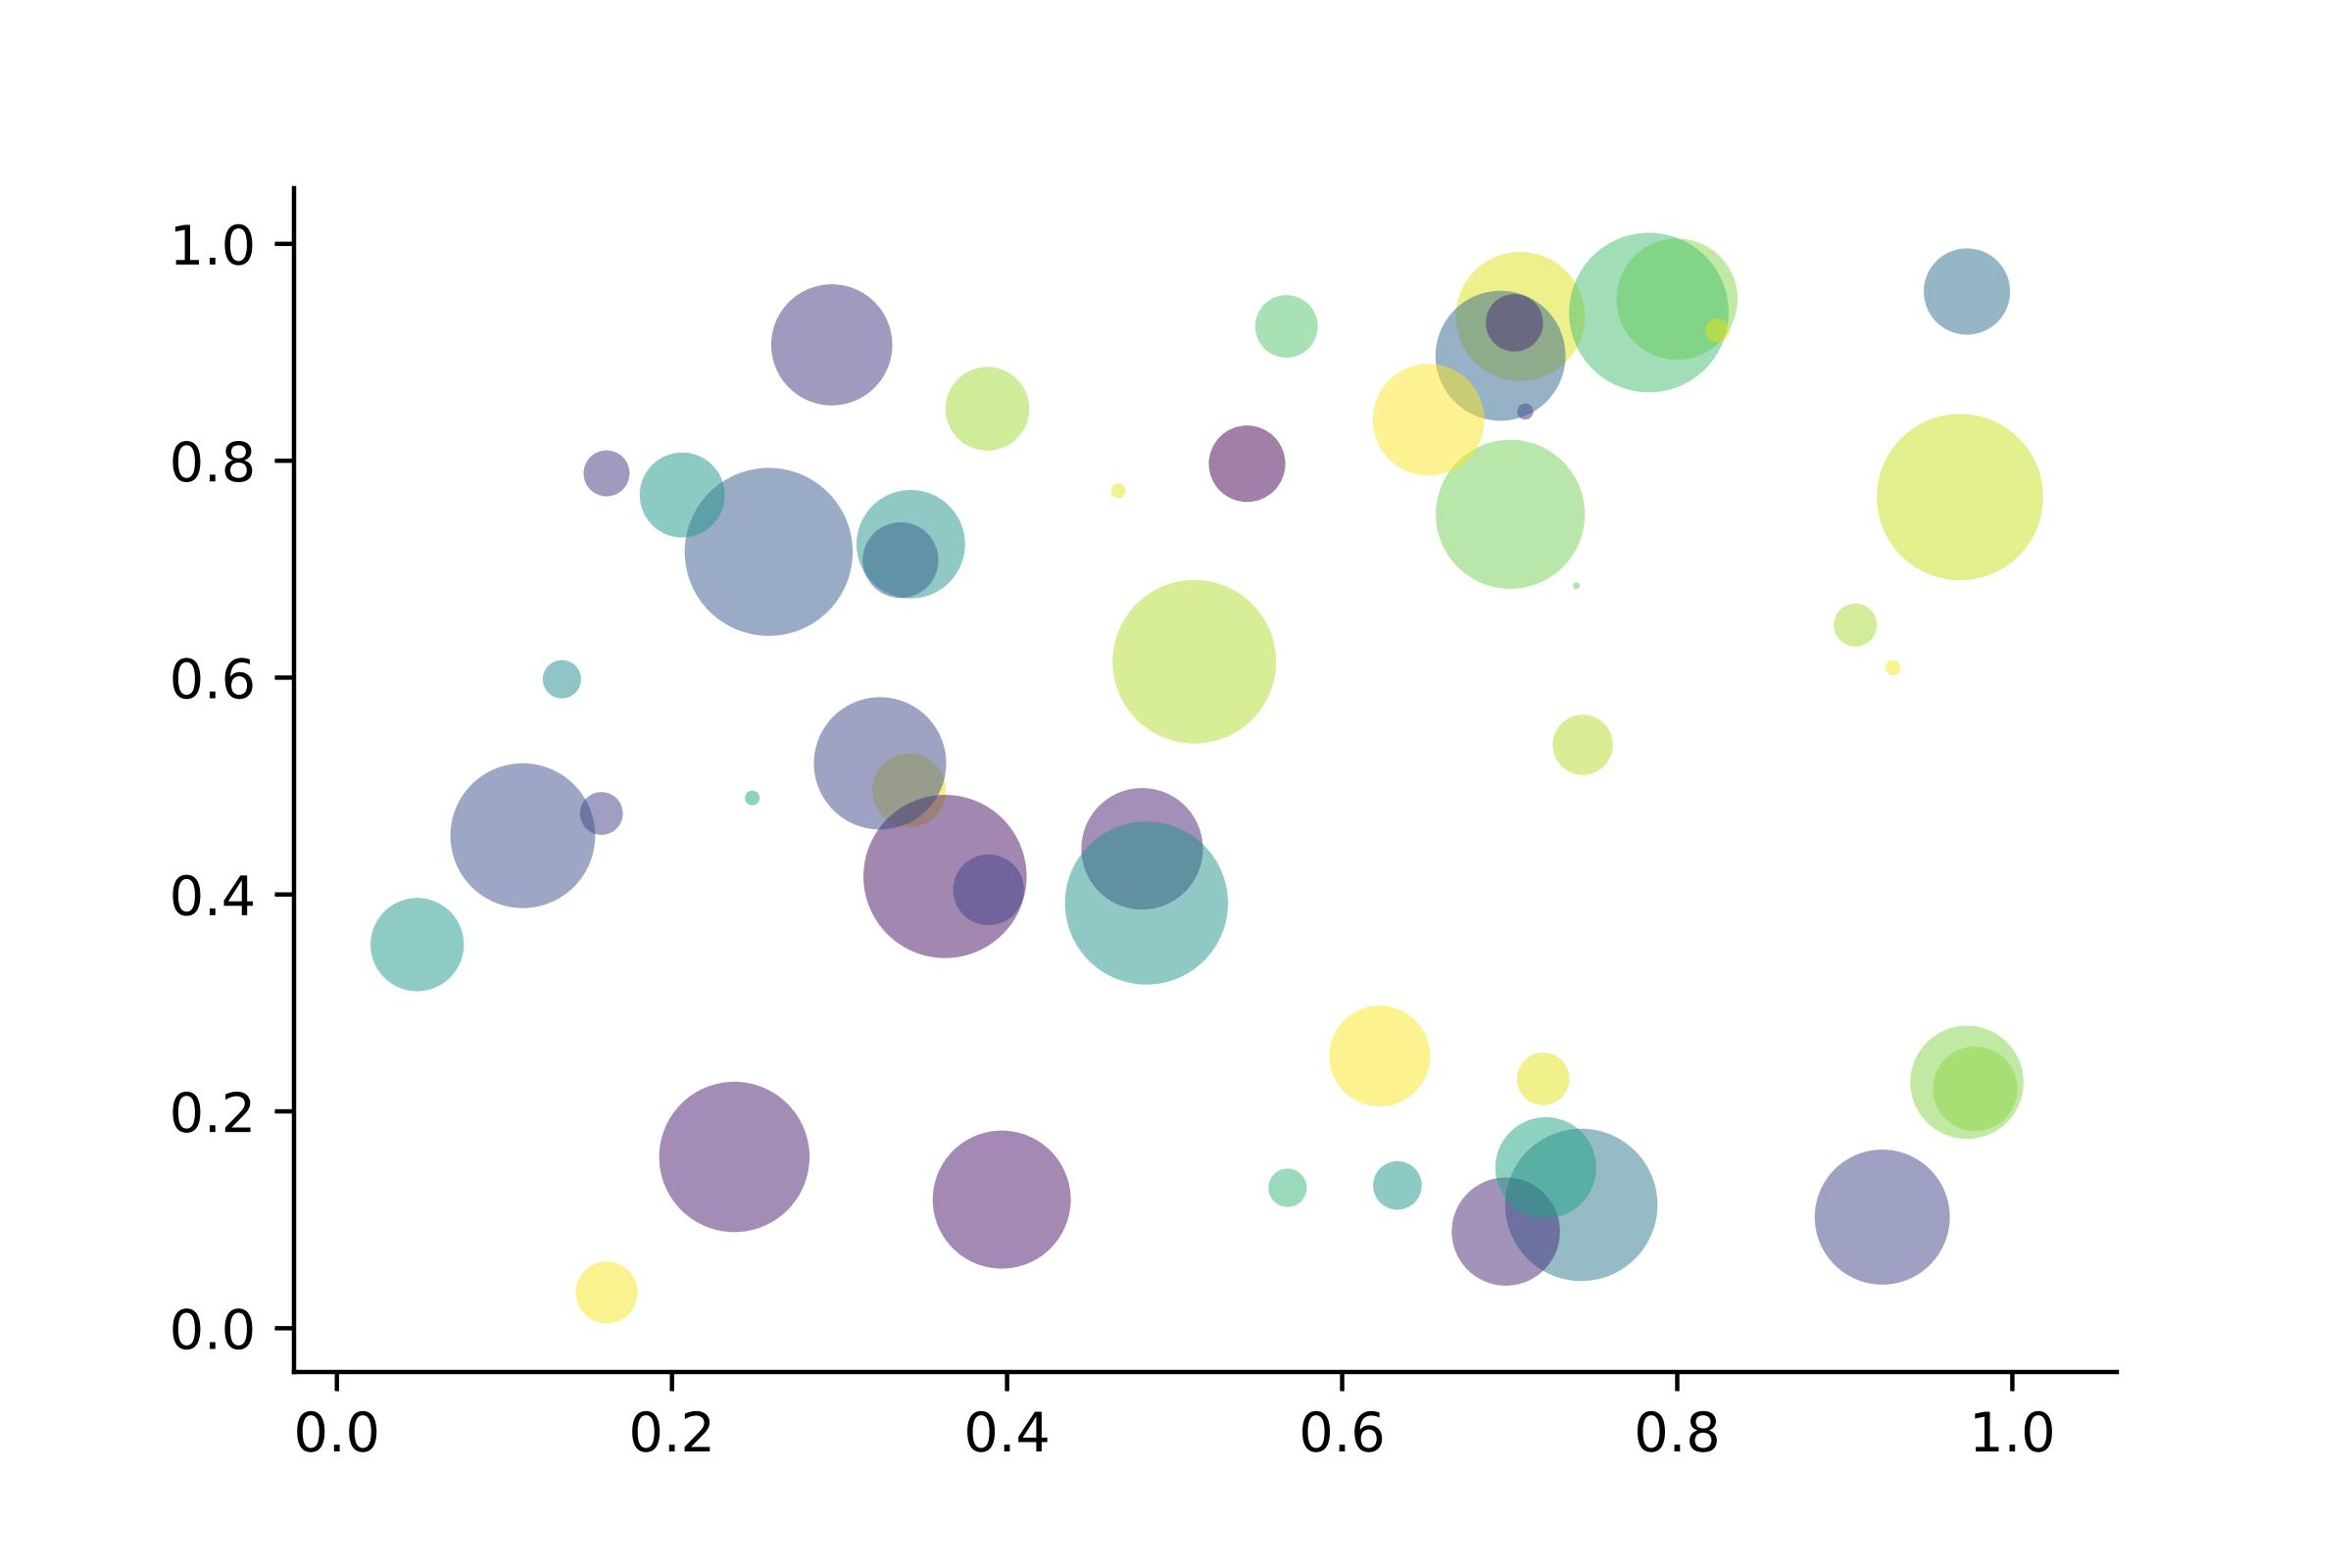
\includegraphics[width=0.6\textwidth]{scatter.jpg}
  \caption{散点图示例 $\hat{y}=a+bx$ \label{fig:scatter}}
\end{figure}

以最简单的一元线性模型来解释最小二乘法。什么是一元线性模型呢?监督学习中,如果预测的变量是离散的,我们称其为分类(如决策树,支持向量机等),如果预测的变量是连续的,我们称其为回归。回归分析中,如果只包括一个自变量和一个因变量,且二者的关系可用一条直线近似表示,这种回归分析称为一元线性回归分析。如果回归分析中包括两个或两个以上的自变量,且因变量和自变量之间是线性关系,则称为多元线性回归分析。对于二维空间线性是一条直线;对于三维空间线性是一个平面,对于多维空间线性是一个超平面。

\begin{property}\label{property:cauchy}
柯西列的性质
\begin{enumerate}
\item $\{x_k\}$ 是柯西列,则其子列 $\{x_k^i\}$ 也是柯西列。
\item $x_k\in \mathcal{R}^n$,$\rho(x,y)$ 是欧几里得空间,则柯西列收敛,$(\mathcal{R}^n,\rho)$ 空间是完备的。
\end{enumerate}
\end{property}

\begin{conclusion}
回归分析(regression analysis) 是确定两种或两种以上变量间相互依赖的定量关系的一种统计分析方法。运用十分广泛,回归分析按照涉及的变量的多少,分为一元回归和多元回归分析;按照因变量的多少,可分为简单回归分析和多重回归分析;按照自变量和因变量之间的关系类型,可分为线性回归分析和非线性回归分析。
\end{conclusion}

\begin{problemset}
\item 设 $A$ 为数域 $K$ 上的 $n$ 级矩阵。证明:如果 $K^n$ 中任意非零列向量都是 $A$ 的特征向量,则 $A$ 一定是数量矩阵。
\item 证明:不为零矩阵的幂零矩阵不能对角化。
\item 设 $A = (a_{ij})$ 是数域 $K$ 上的一个 $n$ 级上三角矩阵,证明:如果 $a_{11} = a_{22} = \cdots = a_{nn}$,并且至少有一个 $a_{kl} \not = 0 (k < l)$,则 $A$ 一定不能对角化。
\end{problemset}

\chapter{常见问题集}


\nocite{*}
\printbibliography[heading=bibintoc, title=\ebibname]
\appendix

\chapter{基本数学工具}


本附录包括了计量经济学中用到的一些基本数学,我们扼要论述了求和算子的各种性质,研究了线性和某些非线性方程的性质,并复习了比例和百分数。我们还介绍了一些在应用计量经济学中常见的特殊函数,包括二次函数和自然对数,前 4 节只要求基本的代数技巧,第 5 节则对微分学进行了简要回顾;虽然要理解本书的大部分内容,微积分并非必需,但在一些章末附录和第 3 篇某些高深专题中,我们还是用到了微积分。

\section{求和算子与描述统计量}

\textbf{求和算子} 是用以表达多个数求和运算的一个缩略符号,它在统计学和计量经济学分析中扮演着重要作用。如果 $\{x_i: i=1, 2, \ldots, n\}$ 表示 $n$ 个数的一个序列,那么我们就把这 $n$ 个数的和写为:

\begin{equation}
\sum_{i=1}^n x_i \equiv x_1 + x_2 +\cdots + x_n
\end{equation}



\end{document}
